\documentclass{beamer}
 
\usepackage[utf8]{inputenc}
\usepackage{epstopdf}
\usepackage{graphicx}
%Information to be included in the title page:
\title{Coordinate Geometry}
\subtitle{A Matrix approach}
\author{Gautham Gururajan \and Vignatha Vinjam}
\institute{Indian Institute of Technology Hyderabad}
\date{February 2019}
 
 
\begin{document}
 
\frame{\titlepage}
 
\begin{frame}
\frametitle{Problem}
Tangents drawn from the point $\begin{bmatrix}-8\\0
\end{bmatrix}$ to the parabola \newline
$\mathbf{x}^T \begin{bmatrix} 0 & 0 \\0 & 1
\end{bmatrix} \mathbf{x} + \begin{bmatrix} -8 & 0
\end{bmatrix} \mathbf{x} = 0$ \newline
\newline
touch the parabola at \textbf{\textit{A}} and \textbf{\textit{B}}. \newline
\newline
If \textbf{\textit{F}} is the focus of this parabola, find the area of $\Delta \mathbf{ABF}$ 

\end{frame}
\begin{frame}
\frametitle{Introduction}
For a curve $\textbf{S}$, if variables are replaced in accordance to $\textbf{T = 0}$,
\newline 
in coordinate representation, we replace $x$ with $(x+x1)/2$ and $x^{2}$ with $x*x1$, and similarly for variable $y$, to obtain equation of Tangent at point $\begin{bmatrix} x1 & y1
\end{bmatrix}$ on $\textbf{S}$
\newline
\newline
In this problem, we will take the tangent solution as : 
\newline
\newline
$\mathbf{x}^T \begin{bmatrix} 0 & 0 \\0 & 1
\end{bmatrix} \mathbf{x1} + \begin{bmatrix} -8 & 0
\end{bmatrix} \mathbf{(x + x1)/2} = 0$ \newline
\newline
where $\mathbf{x1}$ is the point at which the tangent is drawn.
\end{frame}

\begin{frame}
\frametitle{Approach }
The steps we took to solve this problem were:
\begin{itemize}
	\item<1-> First obtain a constraint from $\textbf{T} = 0$.
	\item<2-> Using this constraint, apply it in the given parabola equation.
	\item<3-> Finally find the required points and calculate the required area.
\end{itemize}

\end{frame}

\begin{frame}
\frametitle{Solution(Approach A)}
\begin{itemize}
	\item<1-> Clearly, the focus of this parabola is $F = \begin{bmatrix} 2 \\ 0
	\end{bmatrix}$, from the standard form
	\item<2-> From the given parabola we calculate the tangent equation as $\mathbf{x}^T \begin{bmatrix} 0 & 0 \\0 & 1
	\end{bmatrix} \mathbf{x1} + \begin{bmatrix} -8 & 0
	\end{bmatrix} \mathbf{(x + x1)/2} = 0$ \newline
	\newline

	\item<3-> Also, it is given that this tangent passes through $\begin{bmatrix} -8 \\ 0
	\end{bmatrix}$.
	\newline
	\newline
	
	\item<4->$ \begin{bmatrix} -8 & 0
	\end{bmatrix}\begin{bmatrix} 0 & 0 \\0 & 1
	\end{bmatrix} \mathbf{x1} + \begin{bmatrix} -4 & 0
	\end{bmatrix} (\mathbf{x1} +\begin{bmatrix} -8 \\ 0
	\end{bmatrix} ) = 0$ \newline
	\newline
\end{itemize}
\end{frame}
\begin{frame}
\frametitle{Solution(Approach A)(Cont.d)}
\begin{itemize}	
	\item<1-> Clearly the first term is a scalar $0$.
	\item<2-> From the second term of the above equation,ie:\newline$\begin{bmatrix} -4 & 0
	\end{bmatrix} (\mathbf{x1} +\begin{bmatrix} -8 \\ 0
	\end{bmatrix} )$ we see that $\mathbf{x1}$ must be of the form $\begin{bmatrix} 8 \\ y
	\end{bmatrix}$ for some $y \in$$ \mathbb{R}$
	\item<3-> Hence, the required points can be derived by putting $\mathbf{x} =\begin{bmatrix} 8 \\ y
	\end{bmatrix} $ in $\mathbf{x}^T \begin{bmatrix} 0 & 0 \\0 & 1
	\end{bmatrix} \mathbf{x} + \begin{bmatrix} -8 & 0
	\end{bmatrix} \mathbf{x} = 0$ \newline
	\newline and hence solving for the $y$ value.
\end{itemize}
\end{frame}
\begin{frame}
\frametitle{Solution(Approach A)(Cont.d)}
\begin{itemize}	
	\item<1-> One easy way to go about this is by making use of python's SymPy library.
	\item<2-> The solution that we have used has much less time complexity($O(n^{2})$)than that of SymPy's Equation Solver($O(n^{3})$), but only an approximate solution is obtained(0.01\% error), which is acceptable in most cases(Accuracy can be increased at the cost of runtime)
	\item<3-> A threshold value is pre-defined and $y$ is made to take values from a reasonable linear space.
	\item<4-> If the calculated matrix product and sum from the previously stated equation falls below this threshold, then that value of $y$ is returned
	\item<5-> The linear space is flipped and the procedure is repeated, since we expect at most 2 values for $y$
	\item<6-> The two values of $y$ are subsequently found, and now we can easily calculate area of the triangle
\end{itemize}
\end{frame}

\begin{frame}
\frametitle{Results}
\begin{itemize}
	\item<1->Using the above method, the points come out to be \newline \newline$\mathbf{A} = \begin{bmatrix} 8 \\ +7.99979997999
	\end{bmatrix} $\newline $\mathbf{B} = \begin{bmatrix} 8 \\ -7.99979997999
	\end{bmatrix}$\newline \newline
	\item<2->The area of $\Delta\mathbf{ABF}$ is hence : \newline \newline
	1/2*$\begin{vmatrix}2 & 0 & 1 \\ 8 & 7.99979997999 & 1 \\ 8 & -7.99979997999 & 1
	\end{vmatrix} = 47.99879987998$ sq. units.
\end{itemize}
\end{frame}


\begin{frame}
\frametitle{Solution(Approach B)}
\begin{itemize}
	\item<1-> We have :\newline \newline $\begin{bmatrix} -4 & 0
	\end{bmatrix} (\mathbf{x1} +\begin{bmatrix} -8 \\ 0
	\end{bmatrix} ) = 0 $
	\item<2->  $\begin{bmatrix} -4 & 0
	\end{bmatrix} \mathbf{x1}$  $ = \begin{bmatrix} 4 & 0
	\end{bmatrix} \begin{bmatrix} -8 \\ 0
	\end{bmatrix}$ or simply \newline \newline $\begin{bmatrix} 4 & 0
	\end{bmatrix} \mathbf{x1}$  $ = 32$ \newline
	\newline
	or $\begin{bmatrix} 1 & 0
	\end{bmatrix} \mathbf{x1}$  $ = 8$
\end{itemize}
\end{frame}

\begin{frame}
\frametitle{Solution(Approach B)(Cont.d)}
\begin{itemize}
	\item<1-> From the question, we have \newline
	$\mathbf{x1}^T \begin{bmatrix} 0 & 0 \\0 & 1
	\end{bmatrix} \mathbf{x1} + \begin{bmatrix} -8 & 0
	\end{bmatrix} \mathbf{x1} = 0$ \newline
	\newline
	\item<2-> On observing carefully, we can see that the matrix $\begin{bmatrix} 0 & 0 \\0 & 1
	\end{bmatrix}$ can be written as  $\begin{bmatrix}0 \\ 1
\end{bmatrix}\begin{bmatrix}0 & 1
\end{bmatrix}$
	\item<3-> So, 
	$\mathbf{x1}^T \begin{bmatrix}0 \\ 1
	\end{bmatrix}\begin{bmatrix}0 & 1
	\end{bmatrix} \mathbf{x1} = \begin{bmatrix} 8 & 0
	\end{bmatrix} \mathbf{x1} $ \newline
	\newline
	\item<4-> And from the previous result, $\begin{bmatrix} 1 & 0
	\end{bmatrix} \mathbf{x1}$  $ = 8$ \newline or, $\begin{bmatrix} 8 & 0
	\end{bmatrix} \mathbf{x1}$  $ = 64$

\end{itemize}
\end{frame}
\begin{frame}
\frametitle{Solution(Approach B)(Cont.d)}
\begin{itemize}
	\item<1-> Let us put $\mathbf{x1}^T \begin{bmatrix}0 \\ 1
	\end{bmatrix}= L$
	(Which is clearly a scalar, on seeing the dimensions $=>$ $L^{T} = L$)
	\item<2-> We see that $LL^{T} = 64$ or $L^{2} = 64$ or $ L^{T} = \pm 8 $
	\item<3-> Or, $\begin{bmatrix} 0 & 1
	\end{bmatrix} \mathbf{x1}$  $ = \pm 8$
	\item<3-> From the previous equations, we  have \newline \newline
	$\begin{bmatrix} 1 & 0
	\end{bmatrix} \mathbf{x1}$  $ = 8$
	\newline \newline
	$\begin{bmatrix} 0 & 1
	\end{bmatrix} \mathbf{x1}$  $ = \pm 8$ \newline
	\item<4-> Or, \newline \newline$\begin{bmatrix} 1 & 0 \\ 0 & 1
	\end{bmatrix} \mathbf{x1}$  $ =  \begin{bmatrix} +8 \\ \pm 8
	\end{bmatrix}$
\end{itemize}
\end{frame}

\begin{frame}
\frametitle{Solution(Approach B)(Cont.d)}
\begin{itemize}
	\item<1-> $\begin{bmatrix} 1 & 0 \\ 0 & 1
	\end{bmatrix} \mathbf{x1}$  $ =  \begin{bmatrix} +8 \\ \pm 8
	\end{bmatrix}$
	\item<2-> $\mathbf{x1}$  $ =  \begin{bmatrix} +8 \\ \pm 8
	\end{bmatrix}\begin{bmatrix} 1 & 0 \\ 0 & 1
	\end{bmatrix}^{-1}$ $ => \mathbf{x1} = \begin{bmatrix} +8 \\ \pm 8
	\end{bmatrix}$
\end{itemize}
\end{frame}

\begin{frame}
\frametitle{Results}
\begin{itemize}
	\item<1->Using the above method, the points come out to be \newline \newline$\mathbf{A} = \begin{bmatrix} +8 \\ +8
	\end{bmatrix} $\newline $\mathbf{B} = \begin{bmatrix} +8 \\ -8
	\end{bmatrix}$\newline \newline
	\item<2->The area of $\Delta\mathbf{ABF}$ is hence : \newline \newline
	1/2*$\begin{vmatrix}2 & 0 & 1 \\ 8 & 8 & 1 \\ 8 & -8 & 1
	\end{vmatrix} = 48$ sq. units.
\end{itemize}
\end{frame}

\begin{frame}
	\frametitle{Plot}
	\begin{figure}[h]
	\centering
	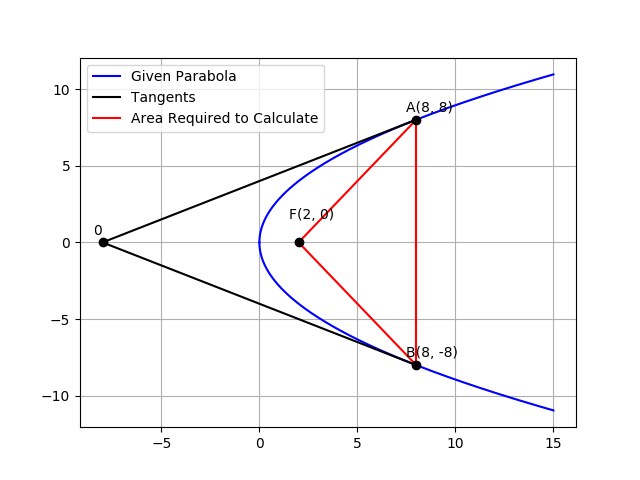
\includegraphics[scale=0.6]{/home/gautham/Desktop/CW/AIML/Fig.png}
	\caption{The Tangents drawn to the parabola, and the required area to be calculated}
	\label{foobar-figure}
	\end{figure}

\end{frame}

\end{document}

